%!TEX root = ../dissertation.tex
\chapter{Experiment 3: Effects of Feedback on Fixational Stability and Accuracy}

\section{Brief Introduction}

Feedback has been identified as an important part of training and skill development for perceptual tasks both similar \citep{vingolo_2007, contestabile_2002} and quite different \citep{pusswald_2013} to ours. Although there is a clear effect of learning evident in both of the previous experiments, their design prevents us from concluding that the \textit{feedback} provided through changes in the gaze-contingent ring's diameter was entirely responsible for the observed effect. Although all subjects were naive to the purposes of the experiment and none were included in both, it is possible that some more general process of task learning was taking place. For this reason, we decided to explicitly compare performance among observers who received feedback from the ring against those performing the same task without feedback.

\section{Methods}

Four Northeastern University undergraduate students were included as participants for this study. All subjects were free of self-reported cognitive and visual deficits, and all had either normal (20/20 Snellen) acuity at baseline, or wore best correction. Subjects were required to read and provide consent to participate by signing an informed consent document. The contents of this document were reviewed and approved by the Northeastern University institutional review board, and were deemed compliant with the terms of the Declaration of Helsinki. The core methodology for this experiment was nearly identical to that used in Experiments 1 and 2, with several modifications to the basic design. First, subjects were only required to complete one training session containing 50 trials, and did not return for a second. The number of trials/training sessions was changed because it was observed in both Experiments 1 and 2 that most of performance enhancement occurred within the first fifty trials of training during the first training session. As with the similar reduction in trial number between Experiments 1 and 2, by constraining our number of trials to this range, we were able to preserve the data quality while further minimizing the experiment's already substantial subject burden (see Figure \ref{chap_3_demo_figure}).

\begin{figure}[!htbp]
\centering
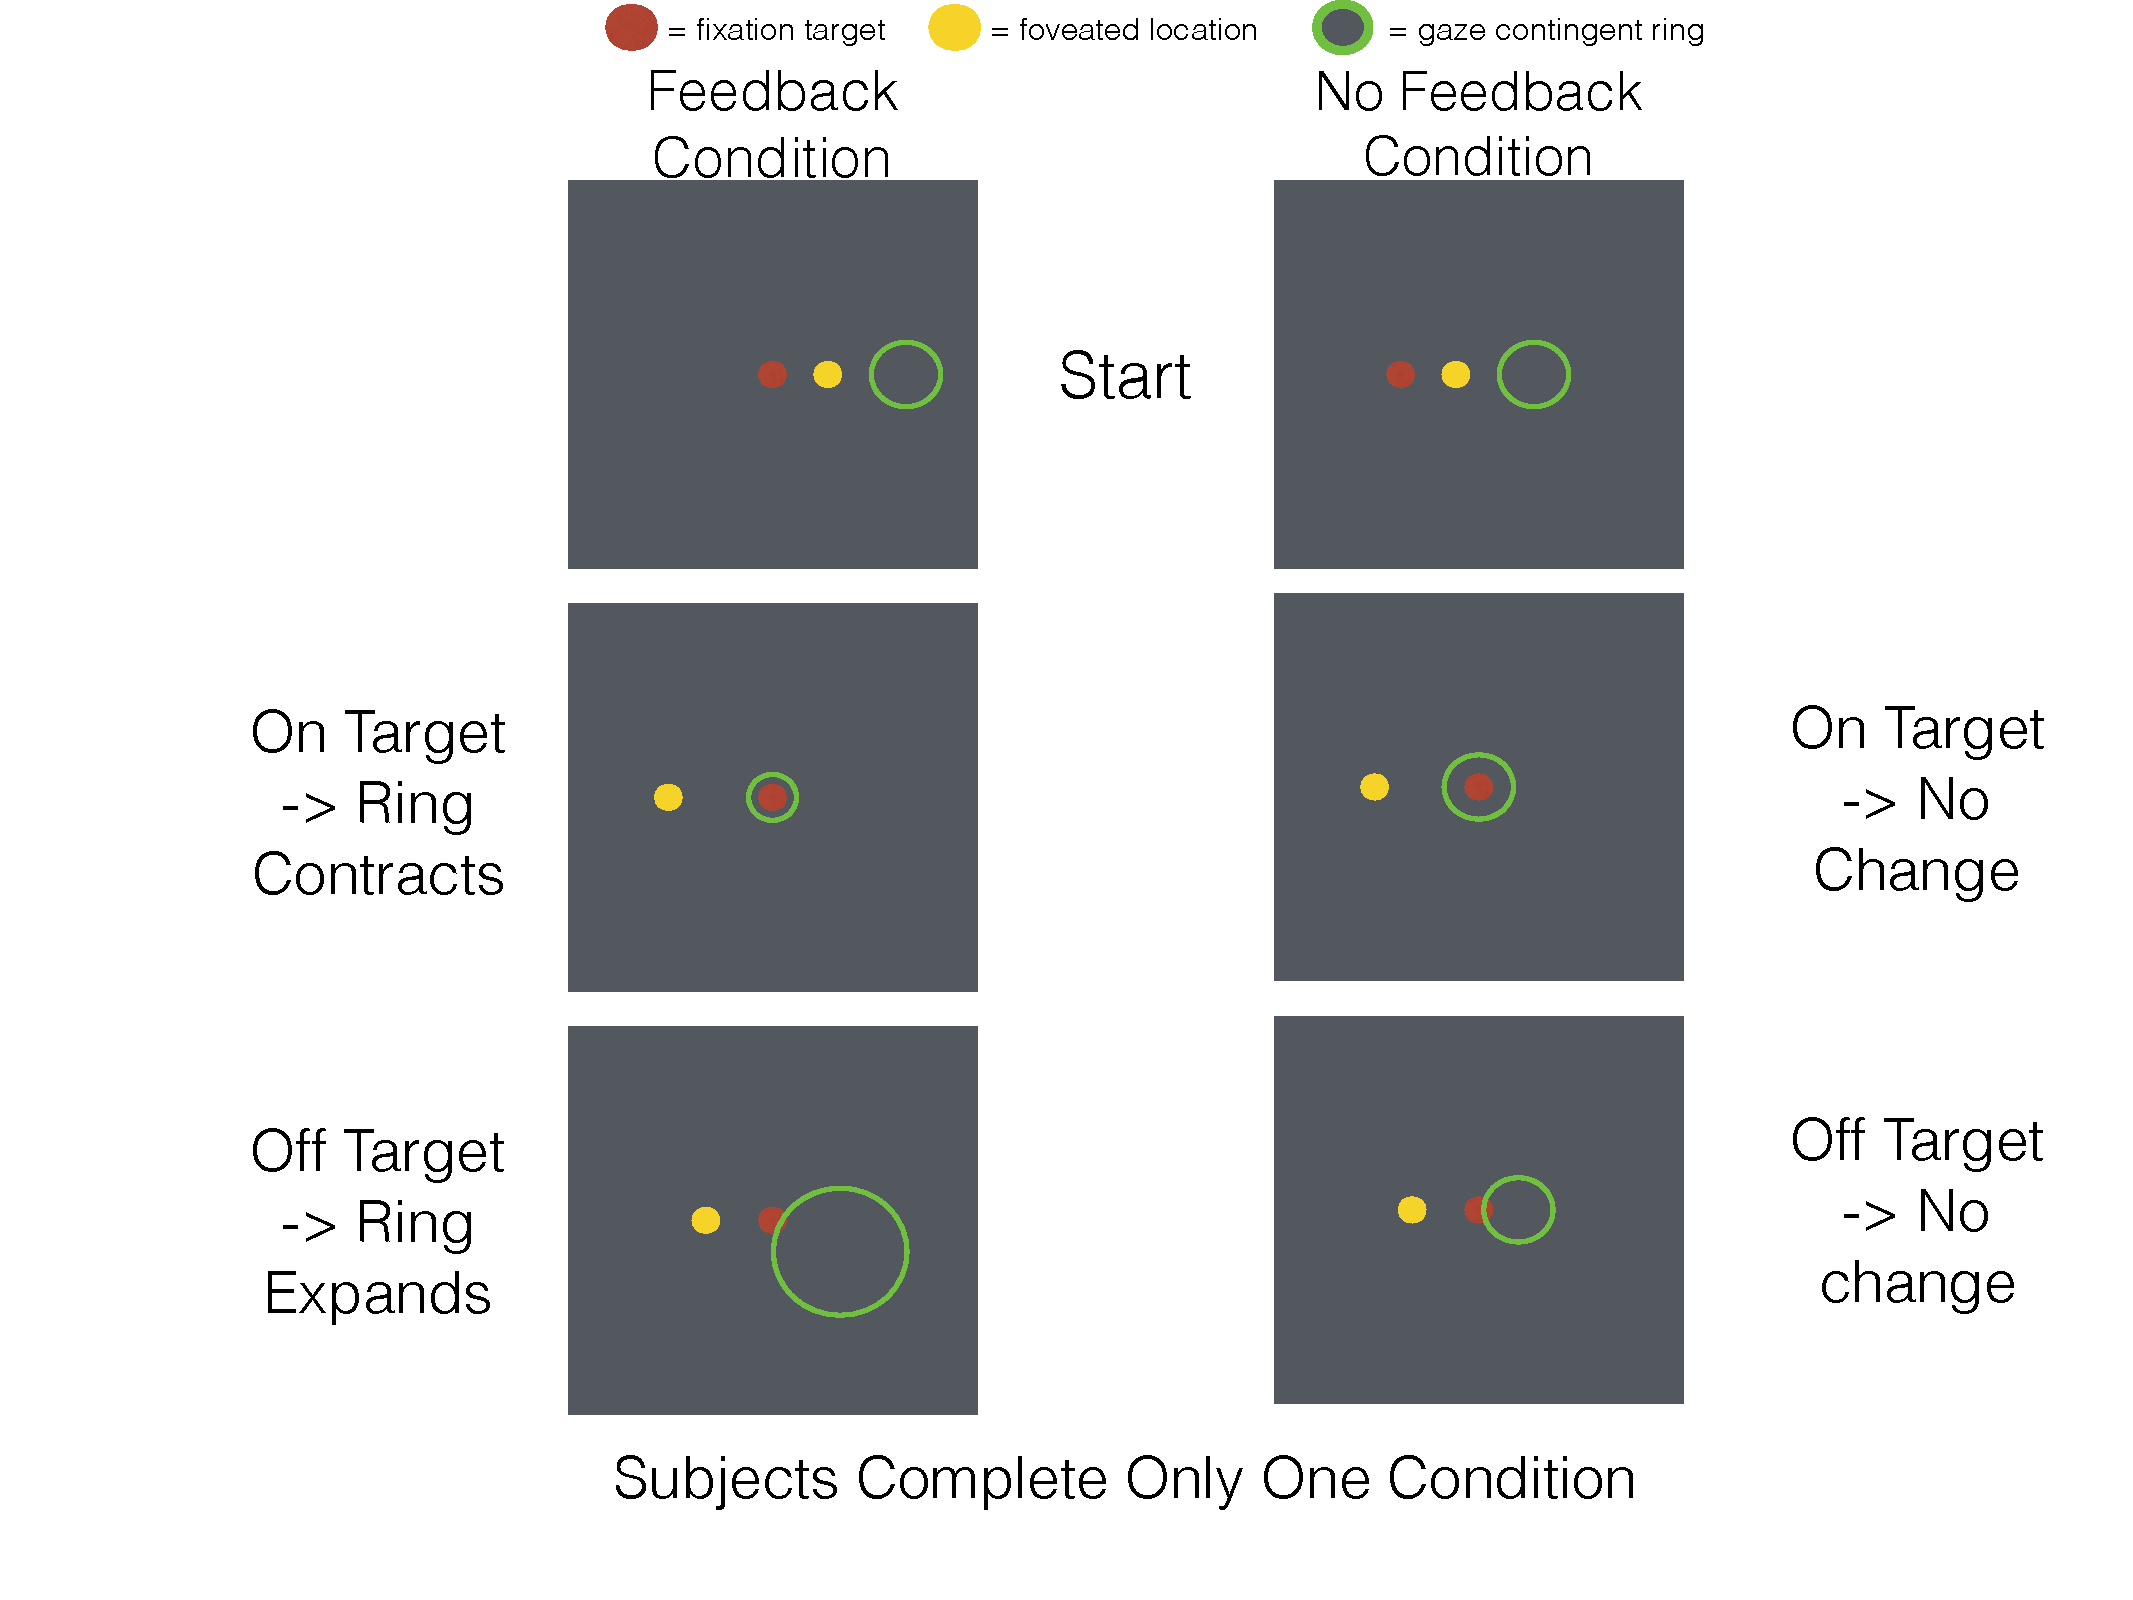
\includegraphics[width=.75\linewidth,height=.75\textheight,keepaspectratio]{figures/chapter_3/feedback_demo.pdf}
\caption[Schematic Depiction of Experimental Design for Experiment 3]{Subjects completed a training session composed of 50 trials in one feedback condition. In the feedback condition, keeping the ring on target caused it to contract after 100ms, making the task harder. Falling off target during the same period caused it to expand, making the task easier. In the no feedback condition, the diameter of the ring was never adjusted as a function of subject's performance. Recorded foveal position (yellow circle) was not shown to research participants.}\label{chap_3_demo_figure}
\end{figure}

The second modification was that no conditional cross was used. All of a subjects' trials were completed within a single condition. In one of the conditions, subjects received feedback on their task performance through adjustment of the diameter of the gaze-contingent ring. In the other, the ring was drawn, but its diameter was \textit{not} adjusted based on performance. In both, the ring was drawn 6.4 degrees to the right of the foveated point of regard. Subjects in the ``no feedback'' condition were given a slightly modified set of task instructions, as it was not possible to ask them to focus on minimizing the diameter of the ring. Instead, they were instructed to simply ``position the center of the green ring as close as possible to the center of the red circle.''

Data from this experiment were again analyzed using \textit{R}. HLMs with a roughly equivalent set of terms to those used for Experiments 1 and 2 were fitted to both sets of outcome data here. The ``time'' or ``learning'' fixed-effect term for this data is \textit{trial} number, not block number, however. Also, as there was no conditional cross, no fixed effect term for training session number or its interaction with condition were included. Finally, because the design of the experiment did not permit us to test retention of learning, no paired t-test for the presence of retention of learning was performed. 

\section{Results}

Figure ~\ref{chap_3_outcome_by_trial} presents aggregated performance for all subjects in each trial for accuracy (\textbf{a}) and stability (\textbf{b}). Performance in terms of both appears to be significantly better for the subjects in the feedback condition than in the no feedback condition; this effect appears to be especially pronounced at the beginning of the training session. 

\begin{figure}[htbp]
\centering
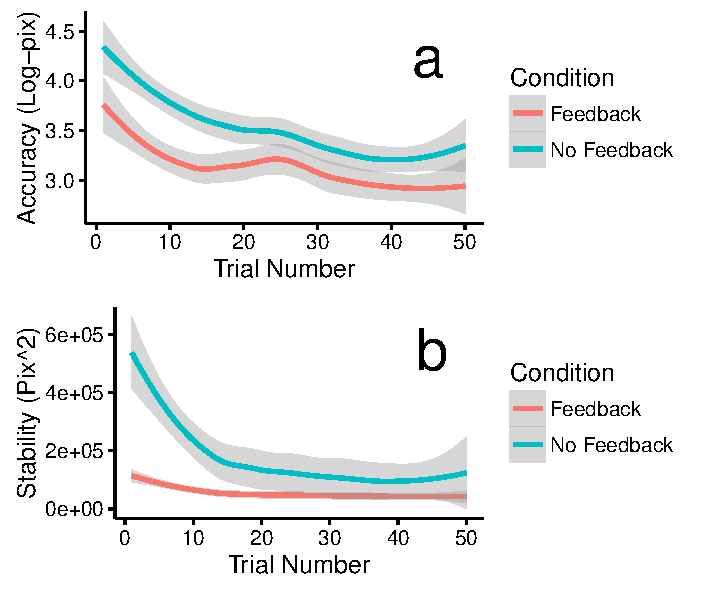
\includegraphics[width=.75\linewidth,height=.75\textheight,keepaspectratio]{figures/chapter_3/outcome_by_trial.pdf}
\caption[Experiment 3: Outcomes by Trial]{\textbf{a}: log-transformed median distance (pixels) between the centers of the target and ring as a function of trial number across subjects. Gray regions are smoothed, LOESS-fitted 95\% confidence bands. \textbf{b}: by-trial stability performance (pixels-squared) across subjects. The elements of this figure are otherwise the same as in \textbf{a}.}\label{chap_3_outcome_by_trial}
\end{figure}

Models fitted to this data (Table ~\ref{chap_3_model_fits}) tell a somewhat more complicated story. For the accuracy data, there were significant main effects of both trial (coefficient: -0.017,\textit{p}\textless0.05) and condition (coefficient: 0.378,\textit{p}\textless0.01), implying that subjects accuracy improved (to a small degree) across trials, and that the absence of feedback made the task significantly more difficult both at baseline and throughout the training. For the stability data, however, only the main effect of feedback condition reached significance (coefficient: 84,353.160,\textit{p}\textless0.01). This suggests that although subjects were \textit{less stable} without the feedback at baseline, the two groups did not differ significantly in the extent to which their gaze stabilized as a function of training across trials. 

\begin{table}[!htbp] \centering 
\resizebox{.75\linewidth}{!}{\begin{minipage}{\linewidth}
  \caption{Experiment 3: Outcome Model Fits} 
  \label{chap_3_model_fits} 
\begin{tabular}{@{\extracolsep{5pt}}lcc} 
\\[-1.8ex]\hline 
\hline \\[-1.8ex] 
 & \multicolumn{2}{c}{\textit{Dependent variable:}} \\ 
\cline{2-3} 
\\[-1.8ex] & Accuracy (Log Pixels) & Stability (Pixels Squared) \\ 
\\[-1.8ex] & (1) & (2)\\ 
\hline \\[-1.8ex] 
 Trial & $-$0.017$^{**}$ & $-$4,225.854 \\ 
  & (0.007) & (3,300.735) \\ 
  Feedback Condition & 0.378$^{***}$ & 84,353.160$^{***}$ \\ 
  & (0.058) & (26,351.290) \\ 
 \hline \\[-1.8ex] 
Observations & 150 & 150 \\ 
Log Likelihood & $-$59.017 & $-$1,962.741 \\ 
Akaike Inf. Crit. & 132.034 & 3,939.482 \\ 
Bayesian Inf. Crit. & 153.109 & 3,960.557 \\ 
\hline 
\hline \\[-1.8ex] 
\textit{Note:}  & \multicolumn{2}{r}{$^{*}$p$<$0.1; $^{**}$p$<$0.05; $^{***}$p$<$0.01} \\ 
\end{tabular}
\end{minipage} } 
\end{table} 

\section{Brief Discussion}

Results from Experiment 3 somewhat conflict with those from Experiments 1 and 2. Though accuracy significantly improved as a function of trials, stability did not. This may be attributable to the relatively small sample size or inability to average data across trials and subjects within blocks. Nevertheless, it highlights the fact that stability gains associated with training  are fairly small in comparison to those for accuracy. To some extent, this makes sense. Fixational stability is presumably an established feature of the participant's existing oculomotor control maps, and thus likely to be resistant to manipulation given such a strong neural ``prior''. Accuracy, as we have defined it, is explicitly tied to our experimental method, and is there not necessarily something that has a single clear representation or control circuit in the brain. The gains observed in terms of accuracy may more likely represent growing familiarity with the task than with any sort of generalized perceptual or motor learning. However, the fact that the absence of feedback significantly reduced performance in terms of \textit{both} outcome measures indicates that our approach \textit{does} impact them both. We therefore conclude that the effects observed in the previous two experiments are not simply attributable to some general form of adaptation to the task, but have an effect on the oculomotor control system specifically related to the stabilization of gaze at new locations. 
